% vim: set textwidth=78 autoindent:

% when the revision of a section has been finalized,
% comment out the following line:
%\updatedisclaimer

\section{Vector Data}\label{sec:vectordata}
\begin{tabular}{p{3.5cm}p{6cm}p{6cm}}
\multirow{2}{*}{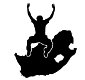
\includegraphics[width=2.5cm]{logo}} & Objectives: &
Understanding of vector data models as used in GIS. \\
& & \\
& Keywords: & 
Vector, Point, Polyline, Polygon, Vertex, Geometry, Scale, Data, Quality,
Symbology, Data Sources  \\
\hline
\end{tabular}

\subsection{Overview}\label{subsec:overview}

\textbf{Vector data} provide a way to represent real world \textbf{features}
within the GIS environment. A feature is anything you can see on the
landscape. Imagine you are standing on the top of a hill. Looking down you
can see houses, roads, trees, rivers, and so on (see Figure
\ref{fig:landscape}). Each one of these things would be a \textbf{feature}
when we represent them in a GIS Application. Vector features have
\textbf{attributes}, which consist of text or numerical information that
\textbf{describe} the features.

\begin{figure}[ht]
   \begin{center}
   \caption{Looking over a landscape you can see the main features, such
as roads, houses and trees.}
\label{fig:landscape}\smallskip
   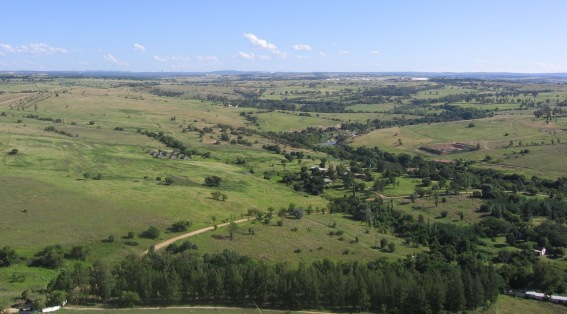
\includegraphics[clip=true, width=\textwidth]{Landscape}
\end{center}
\end{figure}

A vector feature has its shape represented using \textbf{geometry}. The
geometry is made up of one or more interconnected \textbf{vertices}. A vertex
describes a position in space using an \textbf{x}, \textbf{y} and optionally
\textbf{z} axis. Geometries which have vertices with a z axis are often
referred to as \textbf{2.5D} since they describe height or depth at each
vertex, but not both.

When a feature's geometry consists of only a single vertex, it is referred to
as a \textbf{point} feature (see Figure \ref{fig:geometries}a). Where the
geometry consists of two or more vertices and the first and last vertex are
not equal, a \textbf{polyline} feature is formed (see Figure
\ref{fig:geometries}b). Where four or more vertices are present, and the
last vertex is equal to the first, an enclosed \textbf{polygon} feature is
formed (see Figure \ref{fig:geometries}c).

\begin{figure}[ht]
\centering
\caption{Vector point, polyline and polygon geometries}\label{fig:geometries}
   \subfigure[A point feature is described by its X, Y and optionally Z
    coordinate. The point attributes describe the point e.g. if it is a tree
    or a lamp post.]
   {\label{subfig:pointgeo}\fbox{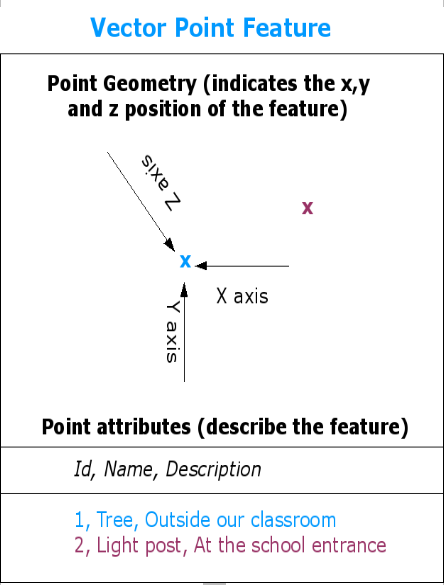
\includegraphics[clip=true, width=0.3\textwidth]{pointgeometry}}}\goodgap
   \subfigure[A polyline is a sequence of joined vertices. Each vertex has an
    X, Y (and optionally Z) coordinate. Attributes describe the polyline.]
    {\label{subfig:linegeo}\fbox{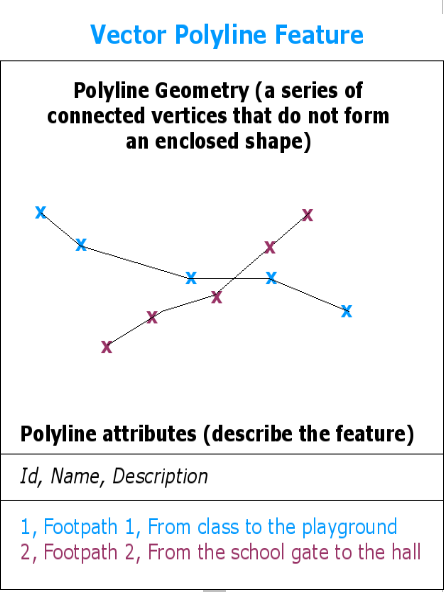
\includegraphics[clip=true, width=0.3\textwidth]{linegeometry}}}\goodgap
   \subfigure[A polygon, like a polyline, is a sequence of vertices. However
    in a polygon, the first and last vertices are always at the same position.]
    {\label{subfig:polygeo}\fbox{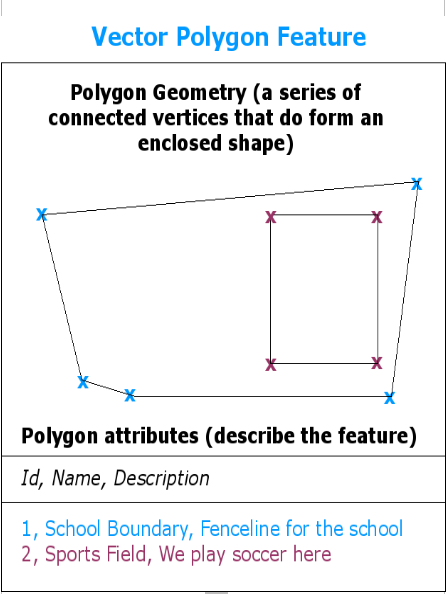
\includegraphics[clip=true, width=0.3\textwidth]{polygongeometry}}}\goodgap
\end{figure}

Looking back at the picture of a landscape we showed you further up, you
should be able to see the different types of features in the way that a GIS
represents them now (see Figure \ref{fig:landscapefeatures}).

\subsection{Point features in detail}\label{subsec:poifeatures}

The first thing we need to realise when talking about point features is that
what  we describe as a point in GIS is a matter of opinion, and often
dependent on scale. let's look at cities for example. If you have a small
scale map (which covers a large area), it may make sense to represent  a city
using a point feature. However as you zoom in to the map, moving towards a
larger scale, it makes more sense to show the city limits as a polygon.

When you choose to use points to represent a feature is mostly a matter of
scale (how far away are you from the feature), convenience (it takes less
time and effort to create point features than polygon features), and the type
of feature (some things like telephone poles just don't make sense to be
stored as polygons).

\begin{figure}[ht]
   \begin{center}
   \caption{Landscape features as we would present them in a GIS. Rivers
(blue) and roads (green) can be represented as lines, trees as points (red)
and houses as polygons (white).}
\label{fig:landscapefeatures}\smallskip
   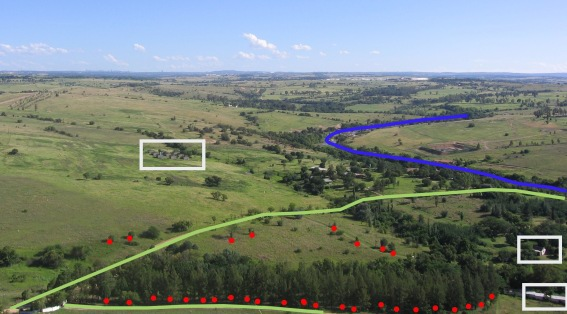
\includegraphics[clip=true, width=\textwidth]{LandscapeFeaturesHighlighted}
\end{center}
\end{figure}

As we show in Illustration 2, a point feature has an X,Y and optionally, Z
value. The X and Y values will depend on the \textbf{Coordinate Reference
System} (CRS) being used. We are going to go into more detail about Coordinate
Reference Systems in a later tutorial. For now let's simply say that a CRS is
a way to accurately describe where a particular place is on the earth's
surface. One of the most common reference systems is \textbf{Longitude and
Latitude}.
Lines of Longitude run from the North Pole to the South Pole. Lines of
Latitude run from the East to West. You can describe precisely where you are
at any place on the earth by giving someone your Longitude (X) and Latitude
(Y). If you make a similar measurement for a tree or a telephone pole and
marked it on a map, you will have created a point feature. 

Since we know the earth is not flat, it is often useful to add a Z value to a
point feature. This describes how high above sea level you are. 

\subsection{Polyline features in detail}\label{subsec:linefeatures}

Where a point feature is a single vertex, \textbf{a polyline has two or more
vertices}. The polyline is a continuous path drawn through each vertex, as
shown in Illustration 3 above). When two vertices are joined, a line is
created. When more than two are joined, they form a 'line of lines', or
\textbf{polyline}.

A polyline is used to show the geometry of \textbf{linear features} such as
roads, rivers, contours, footpaths, flight paths and so on. Sometimes we have
special rules for polylines in addition to their basic geometry. For example
contour lines may touch (e.g. at a cliff face) but should never cross over
each other. Similarly, polylines used to store a road network should be
connected at intersections. In some GIS applications you can set these
special rules for a feature type (e.g. roads) and the GIS will ensure that
these polylines always comply to these rules.

If a curved polyline has very large distances between vertices, it may appear
\textbf{angular} or jagged, depending on the scale at which it is viewed
(see Figure \ref{fig:angularlines}). Because of this it is important that
polylines are digitised (captured into the computer) with distances between
vertices that are small enough for the scale at which you want to use the data.

The \textbf{attributes} of a polyline decribe its properties or
characteristics. For example a road polyline may have attributes that
describe whether it is surfaced with gravel or tar, how many lanes it has,
whether it is a one way street, and so on. The GIS can use these attributes
to symbolise the polyline feature with a suitable colour or line style.

\begin{figure}[ht]
   \begin{center}
   \caption{Polylines viewed at a smaller scale (1:20 000 to the left) may
appear smooth and curved. When zoomed in to a larger scale (1:500 to the
right) polylines may look very angular.}
\label{fig:angularlines}\smallskip
   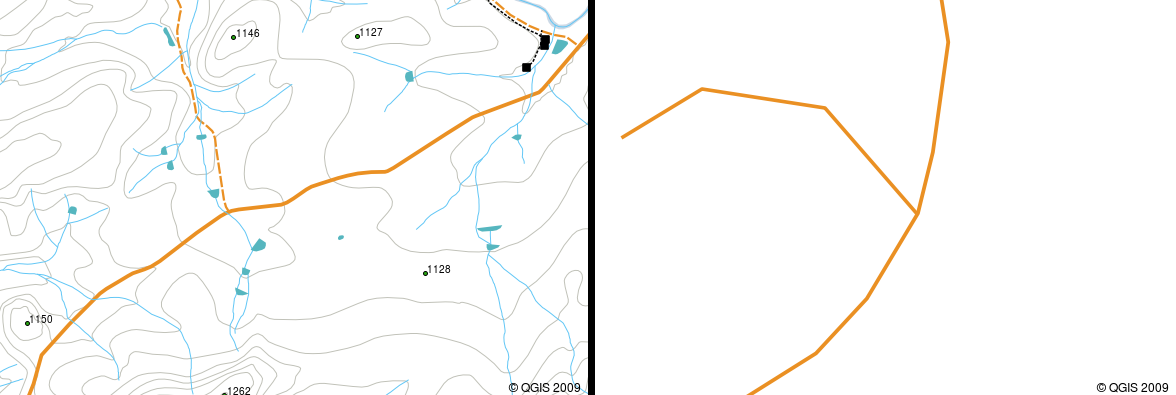
\includegraphics[clip=true, width=\textwidth]{AngularLines}
\end{center}
\end{figure}

\subsection{Polygon features in detail}\label{subsec:polyfeature}

Polygon features are \textbf{enclosed areas} like dams, islands, country
boundaries and so on. Like polyline features, polygons are created from a
series of
vertices that are connected with a continuous line. However because a polygon
always describes an enclosed area, the first and last vertices should always
be at the same place! Polygons often have \textbf{shared geometry} -
boundaries that
are in common with a neighbouring polygon. Many GIS applications have the
capability to ensure that the boundaries of neighbouring polygons exactly
coincide. We will explore this in the \textbf{topology} topic later in this
tutorial.

As with points and polylines, polygons have \textbf{attributes}. The
attributes
describe each polygon. For example a dam may have attributes for depth and
water quality. 

\subsection{Vector data in layers}\label{subsec:vectinlayer}

Now that we have described what vector data is, let's look at how vector data
is managed and used in a GIS environment. Most GIS applications group vector
features into \textbf{layers}. Features in a layer have the the same geometry
type
(e.g. they will all be points) and  the same kinds of attributes (e.g.
information about what species a tree is for a trees layer). For example if
you have recorded the positions of all the footpaths in your school, they
will usually be stored together on the computer hard disk and shown in the
GIS as a single layer. This is convenient because it allows you to hide or
show all of the features for that layer in your GIS application with a single
mouse click.

\subsection{Editing vector data}\label{subsec:editvector}

The GIS application will allow you to create and modify the geometry data in
a layer - a process called \textbf{digitising} - which we will look at more
closely in
a later tutorial. If a layer contains polygons (e.g. farm dams), the GIS
application will only allow you to create new polygons in that layer.
Similarly if you want to change the shape of a feature, the application will
only allow you to do it if the changed shape is correct. For example it won't
allow you to edit a line in such a way that it has only one vertex - remember
in our discussion of lines above that all lines must have at least two
vertices.

Creating and editing vector data is an important function of a GIS since it
is one of the main ways in which you can create personal data for things you
are interested in. Say for example you are monitoring pollution in a river.
You could use the GIS to digitise all outfalls for storm water drains (as
point features). You could also digitise the river itself (as a polyline
feature). Finally you could take readings of pH levels along the course of
the river and digitise the places where you made these readings (as a point
layer).  

As well as creating your own data, there is a lot of free vector data that
you can obtain and use. For example, you can obtain vector data that appears
on the 1:50 000 map sheets from the Chief Directorate : Surveys and Mapping.

\subsection{Scale and vector data}\label{subsec:vectorscale}

Map \textbf{scale} is an important issue to consider when working with vector
data in
a GIS. When data is captured, it is usually digitised from existing maps, or
by taking information from surveyor records and global positioning system
devices. Maps have different scales, so if you import vector data from a map
into a GIS environment (for example by digitising paper maps), the digital
vector data will have the same scale issues as the original map. This effect
can be seen in Figure \ref{fig:mapscales}. Many issues can arise from making
a poor choice of map scale. For example using the vector data in Figure
\ref{fig:mapscales}a to plan a wetland conservation area could result in
important parts of the wetland being left out of the reserve! On the other
hand if you are trying to create a regional map, using data captured at
1:1000 000 might be just fine and will save you a lot of time and effort
capturing the data.

\begin{figure}[ht]
\centering
\caption{Maps with different scales}\label{fig:mapscales}
   \subfigure[Vector data (red lines) that was digitised from a small scale
    (1:1000 000) map.]
   {\label{subfig:scale1mio}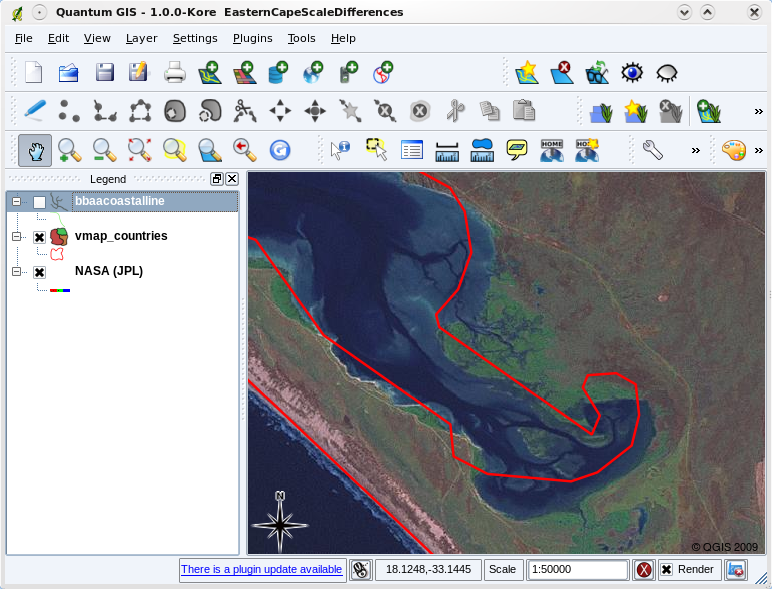
\includegraphics[clip=true, width=0.45\textwidth]{Scale-1mil}}\goodgap
   \subfigure[Vector data (green lines) that was digitised from a large scale
    (1:50 000) map.]
    {\label{subfig:scale50k}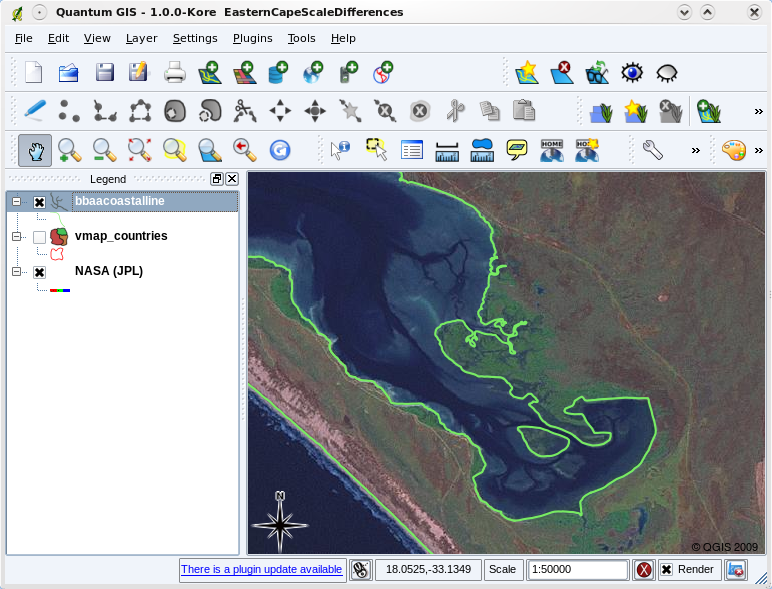
\includegraphics[clip=true, width=0.45\textwidth]{Scale-50k}}\goodgap
\end{figure}

\subsection{Symbology}\label{subsec:symbology}

When you add vector layers to the map view in a GIS application, they will be
drawn with random colours and basic symbols. One of the great advantages of
using a GIS is that you can create personalised maps very easily. The GIS
program will let you choose colours to suite the feature type (e.g. you can
tell it to draw a water bodies vector layer in blue). The GIS will also let
you adjust the symbol used. So if you have a trees point layer, you can show
each tree position with a small picture of a tree, rather than the basic
circle marker that the GIS uses when you first load the layer (see Figure
\ref{fig:symbology}).

Symbology is a powerful feature, making maps come to life and the data in
your GIS easier to understand. In the topic that follows (working with
attribute data) we will explore more deeply how symbology can help the user
to understand vector data.

\begin{figure}[htpb]
\centering
\caption{How can you adjust the symbology of vector features}
   \label{fig:symbology}
   \subfigure[In the GIS, you can use a panel (like the one above) to adjust
    how features in your layer should be drawn.]
    {\label{subfig:symsettings}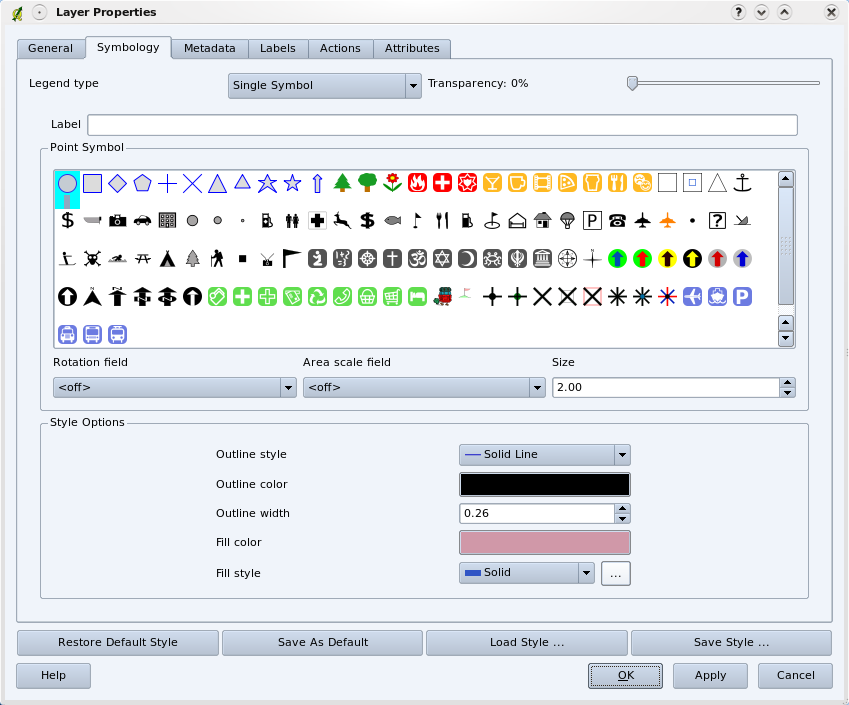
\includegraphics[clip=true, width=0.7\textwidth]{Symbology-settings}} \\
   \subfigure[When a layer (for example the trees layer above) is first
    loaded, a GIS application will give it a generic symbol.]
   {\label{subfig:symdefault}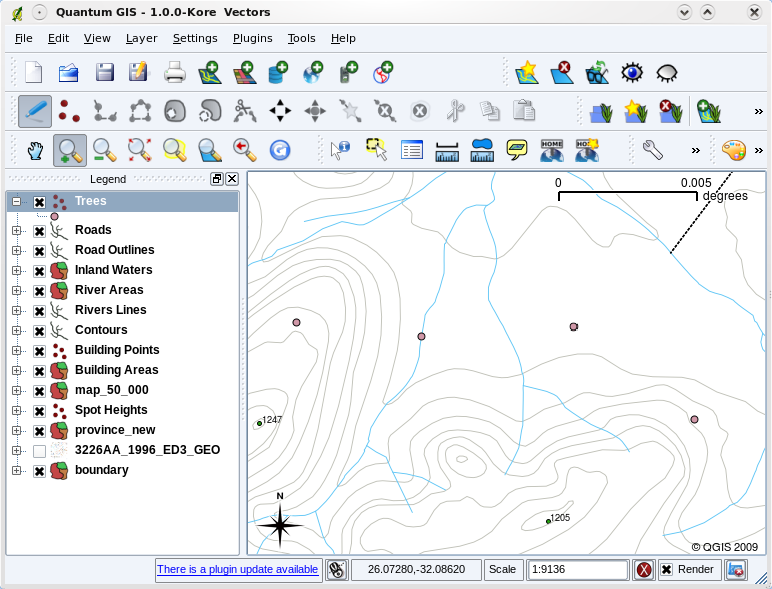
\includegraphics[clip=true, width=0.45\textwidth]{Symbology-default}}\goodgap
   \subfigure[After making our adjustments it is much easier to see that our
    points represent trees.]
    {\label{subfig:symupdate}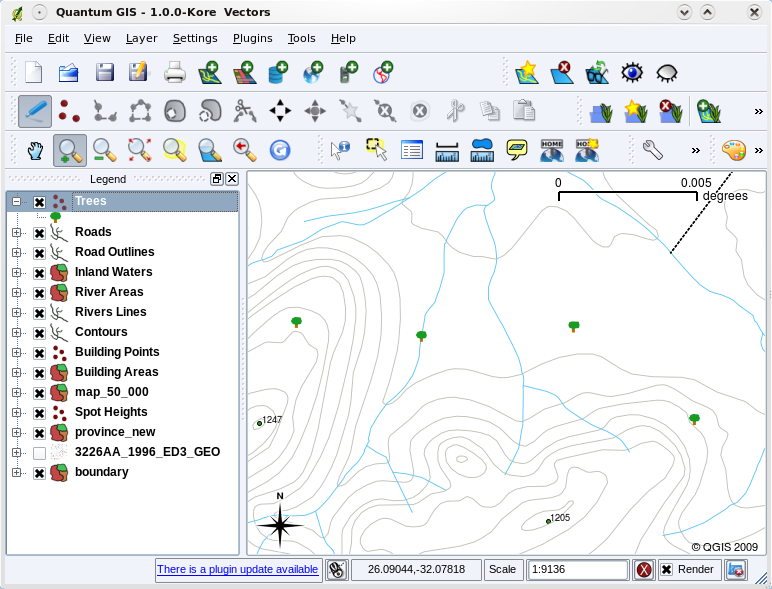
\includegraphics[clip=true, width=0.45\textwidth]{Symbology-updated}}
\end{figure}

\newpage

\subsection{What can we do with vector data in a GIS?}

At the simplest level we can use vector data in a GIS Application in much the
same way you would use a normal topographic map. The real power of GIS starts
to show itself when you start to ask questions like 'which houses are within
the 100 year flood level of a river?'; 'where is the best place to put a
hospital so that it is easily accessible to as many people as possible?';
'which learners live in a particular suburb?'. A GIS is a great tool for
answering these types of questions with the help of vector data. Generally we
refer to the process of answering these types of questions as
\textbf{spatial analysis}. In later topics of this tutorial we will look at
spatial analysis in more detail.

\subsection{Common problems with vector data}

Working with vector data does have some problems. We already mentioned the
issues that can arise with vectors captured at different scales. Vector data
also needs a lot of work and maintenance to ensure that it is accurate and
reliable. Inaccurate vector data can occur when the instruments used to
capture the data are not properly set up, when the people capturing the data
aren't being careful, when time or money don't allow for enough detail in the
collection process, and so on. If you have poor quality vector data, you can
often detect this when viewing the data in a GIS. For example
\textbf{slivers} can
occur when the edges of two polygon areas don't meet properly (see Figure
\ref{fig:slivers}). \textbf{Overshoots} can occur when a line feature such as a
road does not meet another road exactly at an intersection. Undershoots can
occur when a line feature (e.g. a river) does not exactly meet another
feature to which it should be connected. Figure \ref{fig:undershoots}
demonstrates
what undershoots and overshoots look like. Because of these types of errors,
it is very important to digitise data carefully and accurately. In the
upcoming topic on \textbf{topology}, we will examine some of these types of
errors in more detail.

\begin{figure}[ht]
   \begin{center}
   \caption{Slivers occur when the vertices of two polygons do not match
    up on their borders. At a small scale (e.g. 1 on left) you may not be
    able to see these errors. At a large scale they are visible as thin
    strips between two polygons (2 on right).}
\label{fig:slivers}\smallskip
   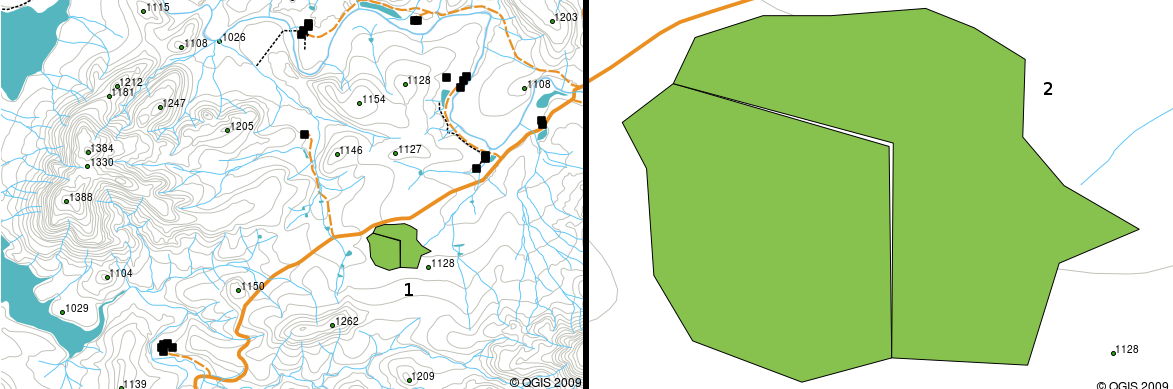
\includegraphics[clip=true, width=\textwidth]{Slivers}
\end{center}
\end{figure}

\begin{figure}[ht]
   \begin{center}
   \caption{Undershoots (1) occur when digitised vector lines that should
    connect to each other don't quite touch. Overshoots (2) happen if a line
    ends beyond the line it should connect to.}
\label{fig:undershoots}\smallskip
   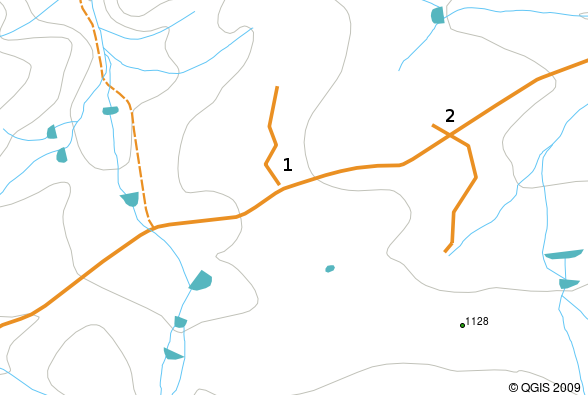
\includegraphics[clip=true, width=0.6\textwidth]{UndershootsOvershoots}
\end{center}
\end{figure}

\subsection{What have we learned?}

Let's wrap up what we covered in this worksheet:

\begin{itemize}
\item \textbf{Vector data} is used to represent real world \textbf{features} in a GIS.
\item A vector feature can have a \textbf{geometry} type of \textbf{point},
\textbf{line} or a \textbf{polygon}.
\item Each vector feature has \textbf{attribute data} that describes it.
\item Feature geometry is described in terms of \textbf{vertices}.
\item Point geometries are made up of a \textbf{single vertex} (X,Y and
optionally Z).
\item Polyline geometries are made up of \textbf{two or more} vertices
forming a connected line.
\item Polygon geometries are made up of \textbf{at least four vertices}
forming an enclosed area. The first and last vertices are always in the same
place.
\item Choosing which geometry type to use depends on scale, convenience and
what you want to do with the data in the GIS.
\item Most GIS applications do not allow you to mix more than one geometry
type in a single layer.
\item Digitising is the process of creating digital vector data by drawing it
in a GIS application.
\item Vector data can have quality issues such as \textbf{undershoots},
\textbf{overshoots} and \textbf{slivers} which you need to be aware of.
\item Vector data can be used for \textbf{spatial analysis} in a GIS
application, for example to find the nearest hospital to a school.
\item We have summarised the GIS Vector Data concept in Figure
\ref{fig:vectordiagram}.
\end{itemize}

\begin{figure}[htpb]
   \begin{center}
   \caption{This diagram shows how GIS applications deal with vector data.}
    \label{fig:vectordiagram}\smallskip
   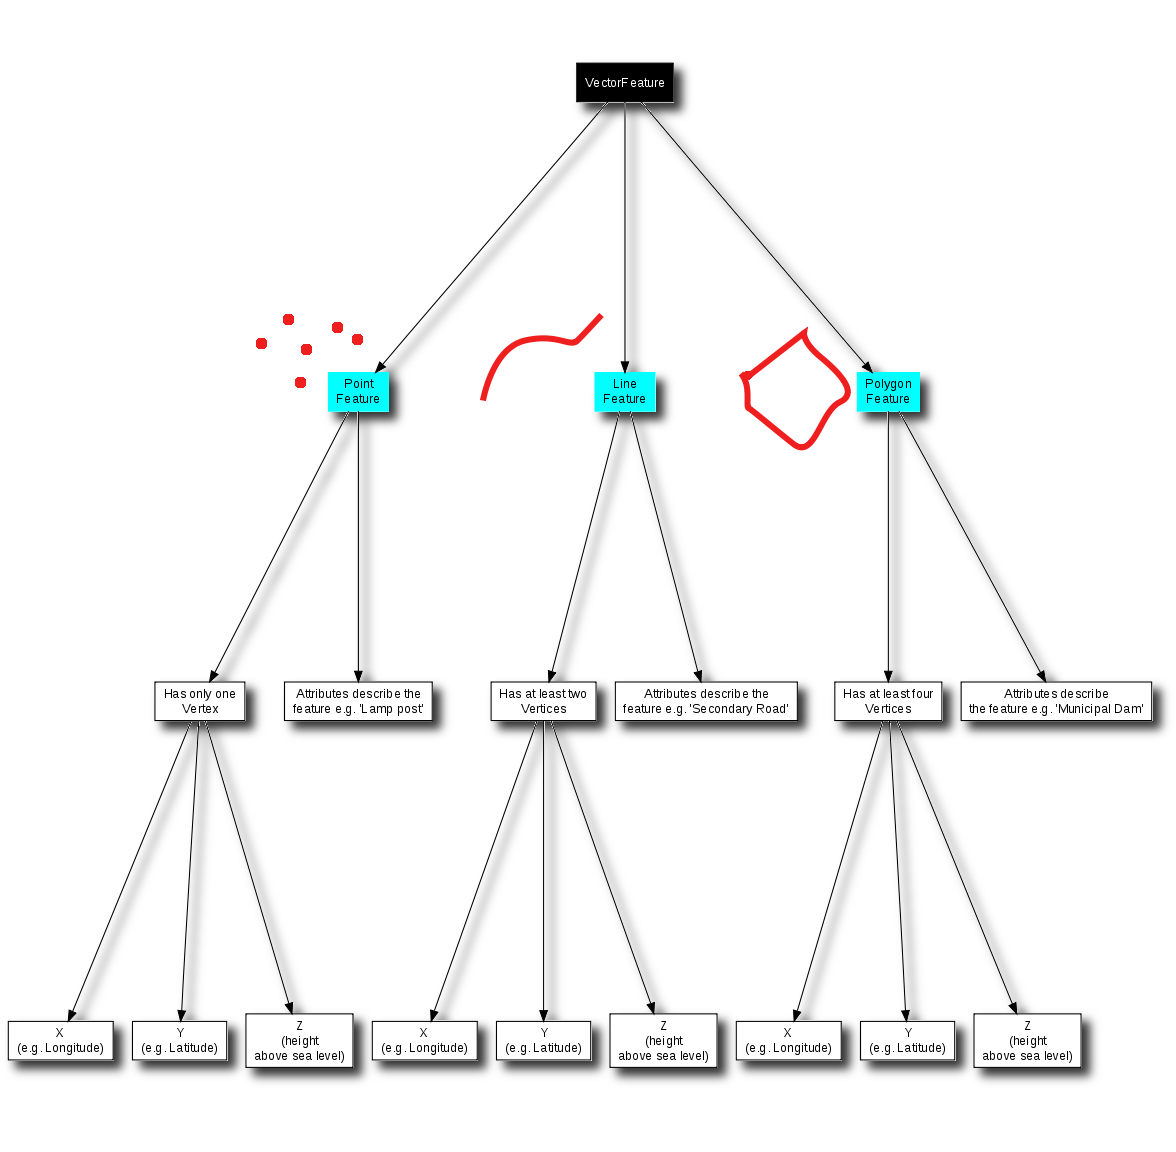
\includegraphics[clip=true, width=\textwidth]{vector_diagram}
\end{center}
\end{figure}

\newpage

\subsection{Now you try!}

Here are some ideas for you to try with your learners:

\begin{itemize}
\item Using a copy of a toposheet map for your local area (like the one shown
in Figure \ref{fig:toposheet}), see if your learners can identify examples of
the different types of vector data by highlighting them on the map.
\item Think of how you would create vector features in a GIS to represent real
world features on your school grounds. Create a table of different features
in and around your school and then task your learners to decide whether they
would be best represented in the GIS as a point, line or polygon. See Table 1
below for an example.
\end{itemize}

\begin{figure}[ht]
   \begin{center}
   \caption{Can you identify two point features and one polygon feature on
    this map?}
    \label{fig:toposheet}\smallskip
   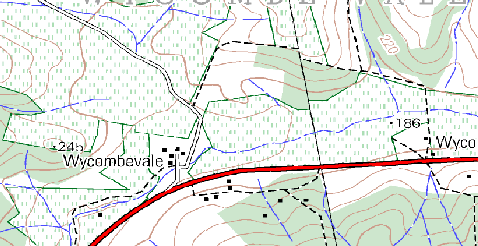
\includegraphics[clip=true, width=0.8\textwidth]{Toposheet}
\end{center}
\end{figure}

%% Note: xdvi does not show white text on black background but it works!
\begin{table}[ht]
\centering
\caption{Create a table like this (leaving the geometry type column empty)
and ask your learners to decide on suitable geometry types.}\medskip
 \label{tab:places}
 \begin{tabular}{|p{8cm}|p{8cm}|}
 \hline
 \rowcolor{black}
 \textcolor{white}{\textbf{Real world feature}} &
 \textcolor{white}{\textbf{Suitable Geometry Type}} \\
 \hline The school flagpole & \\
 \hline The soccer field & \\
 \hline The footpaths in an around the school & \\
 \hline Places where taps are located & \\
 \hline Etc. & \\
\hline
\end{tabular}
\end{table}

\subsection{Something to think about}

If you don't have a computer available, you can use a toposheet and
transparency sheets to show your learners about vector data.

\subsection{Further reading}

The QGIS User Guide also has more detailed information on working with vector
data in QGIS.

\subsection{What's next?}

In the section that follows we will take a closer look at \textbf{attribute
data} to see how it can be used to describe vector features.

